% TEX encoding = UTF-8 Unicode
% Compiled by XeLaTeX.

\documentclass[utf8, a4paper, 11pt, onecolumn]{ctexart}
\usepackage{xeCJK}
\usepackage{setspace}
\usepackage{amsmath}
\usepackage{url}

\title{推荐系统的协同过滤算法实现与浅析}
%\author{}
%\date{\today}

\begin{document}
\begin{spacing}{1.5}

\maketitle
\tableofcontents
\newpage

\end{spacing}

\begin{spacing}{1.25}

\section{项目简介}

个性化推荐系统基于用户的兴趣和商品的特性,向用户推荐合适的信息或商品,其在互联网领域,尤其是电子商务、广告业务等方面,具有非常广泛的应用。推荐系统的进步,会更加迎合用户的需求,会为产品赢得更好的口碑,为企业创造更多的收益,形成良性的循环。因而,对推荐系统算法的研究,在实践中不断发展,不断进步。

本项目选择推荐系统为主题,以协同过滤(Collaborative Filtering)为主要算法,基于MovieLens数据集,采用了交叉验证的方式,以均方根误差RMSE为评价指标。

由于这门课是以算法为核心的课程,因而本项目更加注重算法的具体内容和细节。在项目中,所有核心代码均由自己编写,未调用任何外部算法模块。在报告中,也会主要以算法内容和实现细节为主。

算法以baseline为起步。在baseline的基础上,实现了基本的user-user和item-item协同过滤算法,以及基于baseline的协同过滤算法,验证了item-item相比user-user能获得更好的效果。

同时,在基本的协同过滤算法上,加上了bias、TopK等优化,进一步提升了模型效果。此外,研究了TopK算法中,K的取值对模型效果的影响,以及关于归一化的相似度矩阵对算法效果的影响。最后,尝试融合了不同的算法并调参,获得了更好的融合模型。

在项目过程中,在矩阵计算、相似度处理、评分预测等处,遇到了诸多算法细节问题,并进行了合适的处理。对于矩阵运算的代码,尽量进行了Vectorization,以提高速度。同时,自己重新组织了代码结构,分离了各个功能,使其具有更好的模块性,运行更加流水线化。

所有代码及报告,在隐去个人信息后,开源在GitHub平台(\url{https://github.com/irmowan/Collaborative-Filtering})。代码的使用可参见Readme文件。

\section{平台和工具}

以OS X 10.11及Python 3.5为主要开发环境,使用Anaconda作为Python的科学发行版。

使用Jupyter Notebook作为生产力工具,可以进行方便的调试。

使用Numpy和Pandas作为矩阵运算和数据载入的工具。

使用Matplotlib及Echarts.js作为数据可视化工具。

使用Git作为版本管理的工具。

使用基于Unicode的TeX发行版XeLaTeX撰写报告。

\section{数据摘要}

\subsection{数据集}

原先,我采用的是NetflixPrize 数据集,NetflixPrize是关于电影评分的数据集。标准的NetflixPrize数据集包含了480189个user,和17770个item,以及总计约1亿的ratings。数据集中还包括了打分的时间,以及各部电影id对应的名称和年份。

对于协同过滤方法来说,该数据集产生的评分矩阵规模达$480189 \times 17770$,总元素约有80多亿,在该矩阵上的基本统计已经要耗时数十秒,对该矩阵进行更细粒度的计算则会更慢。

因而,我换用了一个数据格式基本相同,但规模更小的数据集MovieLens\ (\url{http://grouplens.org/datasets/movielens/})。它提供了不同规模的数据集,包括100K, 1M, 10M, 20M(均指Rating数)等多个规模的版本。

此外,相比于NetflixPrize,其提供了更多的信息,除了打分时间以外,包括用户的性别、年龄、职业、地区,以及电影的名称、发行时间、和丰富的标签(科幻、动作、文艺等)。

这些丰富的信息都是可以被推荐系统所利用的。如用户的年龄和职业可以被用来聚类,电影的标签可以用来做基于内容(content-based)的推荐,时间戳可以用来进行时序化的推荐(更新鲜的打分具有更高的权重),这些还可以同协同过滤算法相结合,从而达到提高预测速度和精度的目的。

需要注意的是,MovieLens数据集是经过过滤处理的,所有打分少于20个的用户均被过滤。因而,出现在数据集中的用户,每个用户至少对20部影片进行了打分。(而对于每部影片则不然,可能存在没有被打分的影片)

为了获得较快的执行速度,报告中展示的所有算法的运行结果,均基于100K版本的MovieLens数据集。该数据集包括943 users, 1682 items, 100000 ratings。

\subsection{数据格式与交叉验证}

通过Pandas的DataFrame读入数据。

原先,所有数据采用一组训练集和测试集,训练集和测试集规模比为$4:1$。即,训练集规模为80000,测试集规模为20000。

数据每行格式为(user, item, rating, timestamp),训练集及测试集均为此格式。在测试时,所有测试函数以(user, item)对为输入参数,返回预测的rating。

在读入数据后,由打分数据填充ratings矩阵,以user为行,item为列,形成$943 \times 1682$的矩阵。

为提高指标稳定性,采用了K次交叉验证(K-fold Cross Validation)的方法。将数据切分为5个子样本,每次取4组训练,剩余一组用于测试,循环5次。在交叉意义下的评价指标可见\ref{评价指标}节。

\textit{\textbf{trick}: 数据集内数据id以1开始,内部变量索引以0开始,做适当调整即可。}

\subsection{评价指标}
\label{评价指标}

对于如何评价算法的优劣程度,需要指定相关的评价指标。

一种常见的评价指标是平均绝对误差\textit{Mean Absolute Error}\ (MAE),MAE值越低,则预测效果越好。其定义为:

\[MAE =\frac{\sum_{i=1}^{N} \lvert r_{xi} - \hat{r}_{xi}\rvert}{N} \]

其中,$\hat{r}_{xi}$和$r_{xi}$分别为用户$x$对项目$i$的预测打分及实际打分。MAE值越低,则预测效果越好。

而在项目中,选择了均方根误差\textit{Root Mean Squared Error}\ (RMSE)作为评价指标,它与MAE一样,越低则效果越好。其定义如下:

\[RMSE = \sqrt{\sum_{i = 1}^{N}(r_{xi} - \hat{r}_{xi})^{2}}\]


由于采用了交叉验证的方法,因而选择每组数据集的RMSE均值作为预测方法的最终RMSE值:(k为交叉验证的组数)

\[\overline{RMSE} = \frac{1}{k}\sum_{i=1}^{k}RMSE_{i}\]

\section{模型详解与分析}
\label{模型详解}

\subsection{统计指标及baseline}

首先,对于输入数据进行一些统计分析。

针对矩阵的稀疏程度,只需做简单运算即可得到,打分矩阵的密度为 $5.04\%$。

除零值外,共有五种打分,以某个训练集为例,作出简单的打分分布(图\ref{rating-pie}),可以大致看出各个分数的打分情况。

\begin{figure}[h]
	\centering
	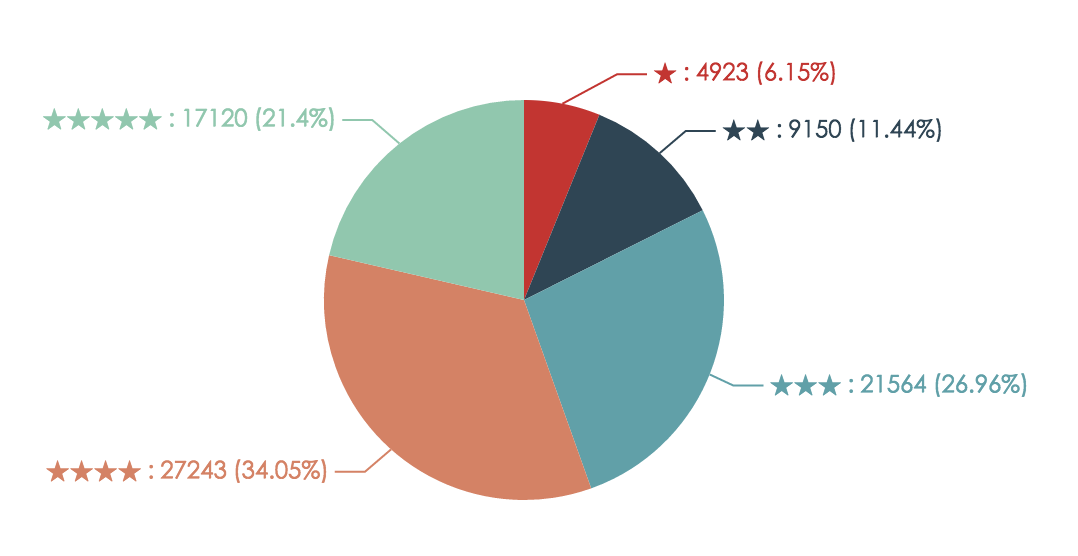
\includegraphics[width=1.0\linewidth]{rating-pie.png}
	\caption{打分分布图}
	\label{rating-pie}
\end{figure}

对矩阵的每一行和每一列求平均值,得到了各个user和item的打分均值。需要注意的是,此处要过滤零值,只对非零值求平均,否则无意义。

\textit{\textbf{trick}: 过滤出非零值不需要每行(列)分别过滤,应采用向量化方法,对整个矩阵执行按行(列)求和和非零值计数运算,直接相除。}

baseline是基于这些统计量的简单预测。其预测公式为

\[\hat{r}_{xi} = \mu + ub_{x} + ib_{i}\]

其中,$\mu$为总体均值,$ub_{x}$和$ib_{i}$分别是user x和item i的均值与总体均值的偏差。化简可得:

\[\hat{r}_{xi} = \overline{r_{user\ x}}+ \overline{r_{item\ i}} - \mu\]

此算法即为baseline的效果,其RMSE值为\textbf{0.9694}.

\textit{\textbf{trick}: numpy采用了float64类型存储浮点数,最好不要对其做任何近似操作,只需在最后的输出结果中采用近似表示即可。}

\subsection{相似度矩阵与协同过滤}

协同过滤(Collaborative filtering)基于这样的思想:如果两个user对大多数item的打分相近,说明这两个user的相似度较高,或者若果两个item被大多数user打分相近,也说明这两个item的相似度较高。

基于相似度的来源,以上分别被称为user-user协同过滤和item-item协同过滤。

相似度采用Cosine距离测量,其公式为:

\[sim(x,y) = \frac{r_x \cdot r_y}{\| r_x \| \| r_y\|}\]

该公式对行和列均有效。其对应的矩阵运算为:

\[Sim = \frac{R \cdot R^T}{\| R\cdot R^T \|}\]

\textit{\textbf{trick}: 为防止divide by zero错误,可以在计算时加上一个小偏差$\epsilon$。即,采用$R\cdot R^T + \epsilon$的方式进行实际计算。}

在得到user相似度和item相似度后,可以通过其相似度矩阵进行预测。

预测公式采用加权平均的方式,为用户对其它item打分和item之间相似度的加权平均(针对item-item协同过滤):

\[\hat{r}_{xi} = \frac{\sum_{j \in N(x)} s_{ij} \cdot r_{xj}}{\sum_{j \in N(x)} s_{ij}} \]

其中$N(x)$为user x打过分的数据。此处不能对所有数据求加权平均,因为其没有打过分的item,求平均值没有意义,反而会增加分母的值,导致预测严重偏差。

\textit{\textbf{trick}:该预测公式还需要一点补充,即冷启动问题,当该公式分母为0时,结果为NaN,此时可以采用baseline结果代替NaN.}

该方法基于item-item的交叉验证结果是\textbf{1.0149},竟然比baseline还高,而基于user-user的结果是\textbf{1.0174},同样超过了1。

\subsection{结合baseline的协同过滤}

所以,baseline的意义是重要的,只采用协同过滤而无视了baseline,效果并没有那么明显。
将baseline和协同过滤结合起来,在baseline的基础上预测,预测公式改为:

\[\hat{r}_{xi} = b_{xi}  + \frac{\sum_{j \in N(x)} s_{ij} \cdot (r_{xj} - b_{xj})}{\sum_{j \in N(x)} s_{ij}} \]

其中,$b_{xi}$为用户x, 项目i的baseline预测值,$N(x)$为用户x打过分的项目集合。同样可以采用向量化计算。

经过改进,基于baseline的item-item协同过滤算法可以将RMSE提高到\textbf{0.9362},相比于baseline有了很大的进步。

而基于baseline的user-user协同过滤也达到了\textbf{0.9548}.

可以得出,在实际应用中,的确item-item的算法表现更加好,大致是商品之间的差异,不如人之间的不同口味差异。

\textit{\textbf{trick}:在进行到此处时,发现了一处细节优化,即由于最终打分必然是1-5的整数值,那么在预测时,若预测结果小于1,可以返回1为结果,若预测结果大于5,则返回5为结果。这个改进是微小但稳健的,其可以将item-item协同过滤RMSE由\textbf{0.9362}提高到\textbf{0.9360}}

\subsection{topK协同过滤与K值的选择}

在协同过滤的预测中,由于需要针对每个预测计算所有的历史数据,时间开销较大,且并不是所有打过分的项目,均属于和item较相似的范畴。因而,可以采取topK技巧,在所有打过分的item中,过滤出与该item相似度最高的K个item,只对这K个item进行加权平均。

\[\hat{r}_{xi} = b_{xi}  + \frac{\sum_{j \in N_k(x)} s_{ij} \cdot (r_{xj} - b_{xj})}{\sum_{j \in N_k(x)} s_{ij}} \]

\textit{\textbf{trick}: 如果用户打过的item数不足K,则直接使用所有打过的item。这也是基于某些用户可能只倾向于对其喜欢的商品评分。}

在运行时,在采用item-item协同过滤的情况下,选择K=10时,得到的RMSE为\textbf{0.9278},选择K=40时,得到的RMSE为\textbf{0.9242}.

可以发现,不同的K值,其效果有一定差异。当K太小时,不能覆盖所有与其较相似的item, 而当K太大时,所选的item可能已经与其不再非常相似。

尝试调整K,对不同的K,得到的RMSE如表格\ref{k-table}.

\begin{table}[t]
	\centering
	\begin{tabular}{| c | c | c | c | c |}
		\hline
		\textbf{K值} & item训练集 & item 测试集&user训练集 & user测试集 \\ 
		\hline
		5 & 0.5747 	& 0.9543 & 0.6101 &	0.9874 \\ 
		\hline
		10 & 0.6845 &	0.9278 & 0.7242 &	0.9573 \\
		\hline
		15 & 0.7322 &	0.9223 & 0.7699 &	0.9489 \\
		\hline
		18 & 0.7500 &	0.9215 &	0.7866 &	0.9468 \\
		\hline
		20 & 0.7596 &	0.9213 & 0.7951 &	0.9458 \\
		\hline
		25 & 0.7774 &	0.9217 &	0.8113 &	0.9449 \\ 
		\hline
		30 & 0.7902 &	0.9225 &	0.8225 &	0.9445 \\
		\hline
		40 &0.8073 &	0.9242 &	0.8373 &	0.9447 \\
		\hline
		50 & 0.8182 &	0.9258 &	0.8465 &	0.9453 \\
		\hline
		100 & 0.8422 & 0.9314 &	0.8660 &	0.9491 \\
		\hline
		200 & 0.8546 &	0.9345 &	0.8747 &	0.9526 \\
		\hline 
	\end{tabular}
	\caption{不同K值下的RMSE}
	\label{k-table}
\end{table}

由表格可以大致看出,此处不同的K值得到的RMSE应该呈现U型。

可以画出对应的RMSE曲线,如图\ref{k-figure}。

\begin{figure}[h]
	\centering
	\includegraphics[width=0.8\linewidth]{k-figure.png}
	\caption{不同K值下的RMSE变化图}
	\label{k-figure}
\end{figure}

由图像中发现,随着K的增大,训练集上的RMSE逐渐增大,而不是一般意义上的逐渐变小。其原因主要是,训练数据融入了均值和相似度,在预测时不可避免地利用到了原先的信息,因而训练集上的RMSE并不具有很强的代表性。

测试集上呈现出非典型的U型,U型的低谷即为对应的最优K值。而在K增大时,其带来的负面作用并没有那么大。这大概是因为,采用更多的数据,边缘数据由于其权重的减少,对最终预测值的影响也减小,类似于经济学中的边际效应递减规律。

显而易见,不同规模的输入,应该要有不同大小的K值相匹配。更大规模的数据,应该需要更大规模的K值。

\textit{\textbf{trick}:在这里,我采用的方式是直接设定一个K值集合,因而对于不同规模不具有很好的适应性。而在实际应用中,更好的方式可以是通过学习的方式,去获得一个较优的K值。}

对于该数据集而言,当采用item-item协同过滤时,K=20为宜,RMSE为\textbf{0.9213},当采用user-user协同过滤时,K=30为宜,RMSE为\textbf{0.9445}.

\subsection{归一化的相似度衡量指标}

在相似矩阵中,除了采用Cosine距离外,还可以有其它的相似度定义。

例如采用Pearson相关系数($Pearson-r$ correlation $corr_{i,j}$)\cite{sarwar2001item},其在算Cosine距离前,首先将同一行(列)的元素减去其平均值,以抹去各人打分标准不同所带来的权重差异,在这个意义下定义了新的相似度矩阵。例如item的相似度计算为:

\[sim(i,j) = \frac{\sum_{u \in U} (r_{ui}-\overline{r_{i}})  (r_{uj}-\overline{r_{j}})} {\sqrt{\sum_{u \in U} (r_{ui}-\overline{r_{i}})^2} \sqrt{\sum_{u \in U} (r_{uj}-\overline{r_{j}})^2}}\]

此即为归一化的相似度矩阵定义。同样,采用向量化方式将加快该矩阵的计算。

而同时用于预测的函数,可以保持不变,仅将其中采用的相似度矩阵换成归一化后的相似度矩阵即可。

然而,在topK item-item协同过滤的基础上,将原先的相似度矩阵替换为归一化后的相似度矩阵,其RMSE反而从\textbf{0.9213}提高到\textbf{0.9253}(k=20)。

至于为什么会出现RMSE反而提高的情况,经与老师讨论及相关查阅后,发现这与数据集本身的一些性质有关,对于某些打分很少的item,做归一化之后,其反而抹去了这些item原来就已经很少的信息。例如一部小众的影片,三四个口味相符的受众同时打出了5分的高分,则归一化之后,一下子抹去了这部电影的高分信息,反而产生了信息的损失。

在这种情况下,那么对于user-user协同过滤,由于该数据集中,每个用户至少打过20个评分,这样的弊端应该会被尽量避免。于是,尝试对user-user协同过滤采用归一化后的相似度矩阵。然而效果同样不尽人意,RMSE从\textbf{0.9445}提高到了\textbf{0.9550}(k=30)。

关于这个问题,草读了相关的几篇论文,发现其主要有两个方面的考虑。

首先,对相似度的度量上,有着广泛的讨论。其中,有一种做法是,依然采用item之间的相似度计算,但是,此时不对item作归一化,而是对user做归一化\cite{sarwar2001item}。

\[sim(i,j) = \frac{\sum_{u \in U} (r_{ui}-\overline{r_{u}})  (r_{uj}-\overline{r_{u}})} {\sqrt{\sum_{u \in U} (r_{ui}-\overline{r_{u}})^2} \sqrt{\sum_{u \in U} (r_{uj}-\overline{r_{u}})^2}}\]

另一种解决方式是,当打分的数量不足时,采用default voting的方法\cite{breese1998empirical}。在这一方法中,使用类似tf-idf的分析法,获得默认的权重值。公式较为复杂:

\[w(u,v) = \frac{\sum_{i} f_{i} \sum_{i} f_{i} r_{u,i} r_{v,i} - (\sum_i f_i r_{u,i}) (\sum_i f_i r_{vi}) }{\sqrt{UV}}\]

其次,由于相似度的衡量方法,在实际使用时,很多本质上很相似的对象,它们的vector distance在Euclidean空间下下可能并不理想\cite{sarwar2001item},这就导致了预测时的偏差。

论文\cite{sarwar2001item}中提出的一种改进是,以线性回归模型的结果,取代简单地使用相似对象的raw rating进行预测。

\[\hat{r}^{'}_{N} = \alpha \hat{r}_i + \beta + \epsilon \]

通过回归的方式,确定公式中的$\alpha$和$\beta$。

\subsection{模型融合与融合参数}

此时,协同过滤算法的各种优化价值似乎已经被压榨完。突然灵光一现,想到NetflixPrize最后的获奖算法,多层次多尺度地融合了三百多个模型\cite{koren2009bellkor}。所以,是否可以借鉴这样的思路,尝试一下模型融合在这种情况下,会产生怎样的效果?

在以上的模型中,在不考虑归一化相似度矩阵的情况下,具有本质区别的方法有两种,item-item协同过滤和user-user协同过滤,虽然来源于同一数据,但它们是两个不同的维度。于是,尝试将这两者相融合。其中,topK算法的K值分别选取20和30,也即其各自的最优值。

对一个测试输入,同时采用两种方法进行预测,并求其均值,也即:

\[\hat{r}_{xi} = \frac{\hat{r_1}_{xi} + \hat{r_2}_{xi}}{2}\]

果真得到了更好的效果,item-item协同过滤的RMSE为\textbf{0.9213}, user-user协同过滤的RMSE为\textbf{0.9445},而融合以后,RMSE降低到了\textbf{0.9176}.

进一步,由于item-item协同过滤的效果更好,所以应该在模型融合时对其采用更大的权重,于是,对融合预测函数作适当修改:

\[\hat{r}_{xi} = 0.6 * \hat{r_1}_{xi} + 0.4 * \hat{r_2}_{xi}\]

得到了更好的RMSE值,为\textbf{0.9159}. 可以看出,模型融合的意义很大。

类似在topK方法中的思路,可以将公式改进为线性融合函数,将融合程度作为预测函数的一个参数:

\[\hat{r}_{xi} = \alpha * \hat{r_1}_{xi} + (1-\alpha) * \hat{r_2}_{xi}\]

其中,$\alpha \in [0, 1]$,在两个端点处即分别退化为两个模型,而系数$\alpha$则表示了融合程度,也即在融合模型中item-item协同过滤的权重。

通过调参,调整$\alpha$的值,可以获得最佳的融合效果。

在不同的$\alpha$值下测量RMSE,得到表\ref{alpha-table}.

\begin{table}[ht]
	\centering
	\begin{tabular}{|c|c|c|}
		\hline
		\textbf{$\alpha$} & 训练集RMSE & 测试集RMSE \\
		\hline
		0.00 & 0.8225 & 0.9445 \\
		\hline
		0.10 & 0.8108 & 0.9368 \\
		\hline
		0.30 & 0.7907 & 0.9248 \\
		\hline
		0.50 & 0.7754 & 0.9176 \\
		\hline
		0.60 & 0.7696 & 0.9159 \\
		\hline
		0.65 & 0.7672 & 0.9155 \\
		\hline
		0.70 & 0.7651 & 0.9154 \\
		\hline
		0.75 & 0.7634 & 0.9156 \\
		\hline
		0.80 & 0.7620 & 0.9161 \\
		\hline
		0.90 & 0.7601 & 0.9181 \\
		\hline
		1.00 & 0.7596 & 0.9213 \\
		\hline
	\end{tabular}
	\caption{不同融合参数$\alpha$下的RMSE}
	\label{alpha-table}
\end{table}

同样,画出不同$\alpha$下,融合模型的RMSE变化趋势(图\ref{alpha-figure})。

\begin{figure}[ht]
	\centering
	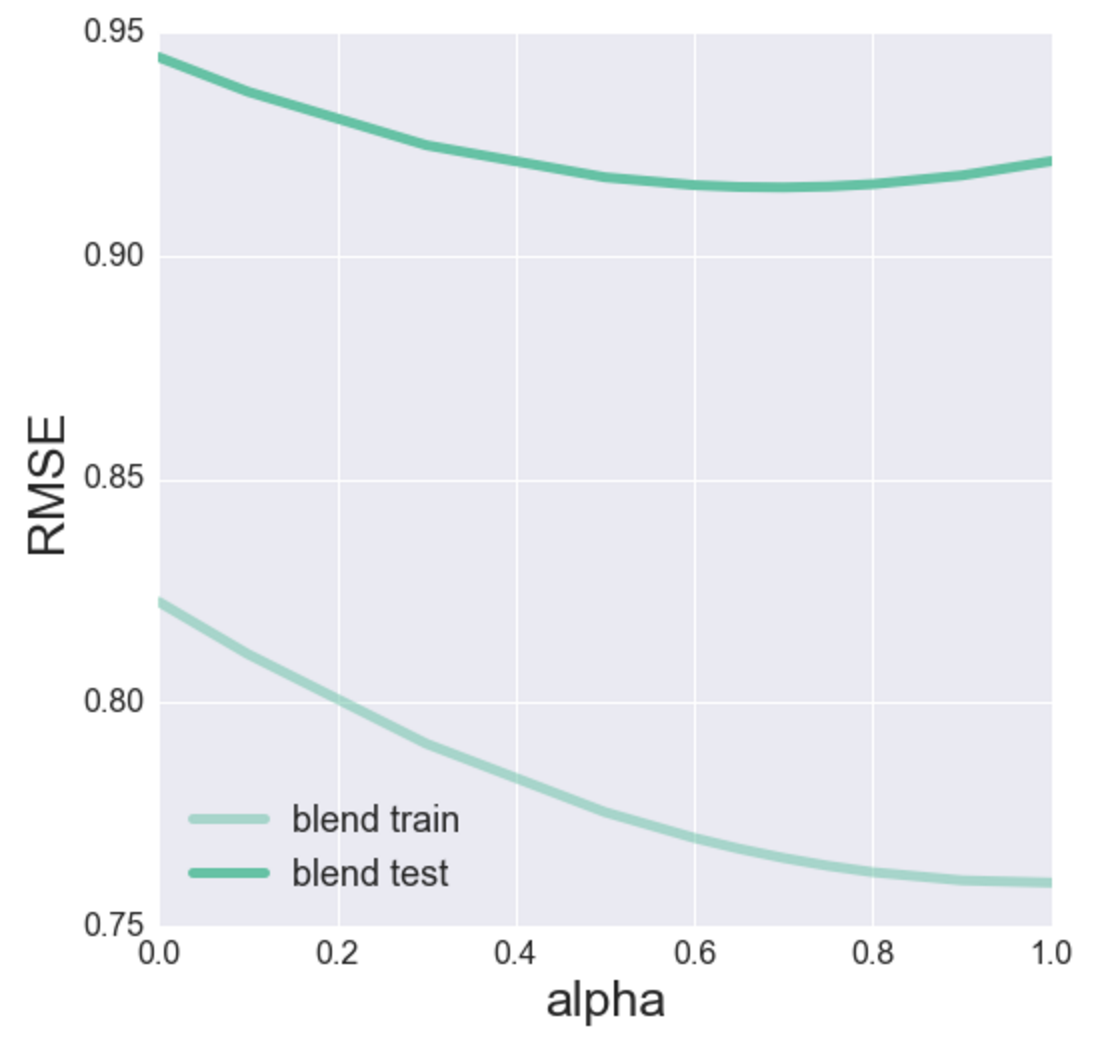
\includegraphics[width=0.8\linewidth]{alpha-figure.png}
	\caption{不同$\alpha$值下的RMSE变化图}
	\label{alpha-figure}
\end{figure}

最终,选取$\alpha = 0.70$,得到了\textbf{0.9154}的RMSE。

此外,还可以考虑一些非线性的模型融合方式。

\subsection{其它算法}

协同过滤被认为是一种基于内存(Memory-based)的推荐算法。它的推荐速度非常快,但由于产生推荐比较耗时,在实时推荐方面还不够有力。

在论文\cite{breese1998empirical}中,作者将还将协同过滤看做是一种概率分布,在这里意义下,一些概率模型就可以发挥其作用,包括Bayesian Classifier, Bayesian Network等。

而在2015年最新的SIGKDD中,论文\cite{wang2015collaborative}将Deep Learning用在协同过滤中,将协同过滤同如今正热的深度神经网络相结合,给推荐系统带来了一些新鲜的活力。

\section{模型结果}

在模型详解一节中,详述了各个算法的定义、公式、相关分析,以及各种trick。

在同一套数据下,利用交叉验证的方式测量不同方法的性能,其最终的RMSE结果为表格\ref{RMSE-table},需要注意的是,这其中很多方法都是建立在前者的方法上,叠加了前面的方法,一点点尝试改进。

\begin{table}[hbtp]
	\centering
	\begin{tabular}{|c|c|}
		\hline
		\textbf{Method} & \textbf{RMSE} \\
		\hline
		baseline &   0.9694 \\
		\hline
		itemCF &  1.0149 \\
		\hline
		userCF & 1.0174 \\
		\hline
		itemCF+baseline &  0.9362 \\
		\hline
		userCF+baseline & 0.9548 \\
		\hline
		itemCF+bias & 0.9360 \\
		\hline
		topkCF(item, k=20) & 0.9213 \\
		\hline
		topkCF(user, k=30) &0.9445 \\
		\hline
		normCF(item, k=20) &0.9253 \\
		\hline
		normCF(user, k=30) &0.9550 \\
		\hline
		blendCF($\alpha$=0.70) & 0.9154 \\		
		\hline
	\end{tabular}
	\caption{不同方法的RMSE比较}
	\label{RMSE-table}
\end{table}

最终,在尝试了各种优化和改进之后,融合了两类协同过滤算法的融合模型取得了\textbf{0.9154}的RMSE值。

\section{总结}

在这个项目中,我以课堂内容为基准,参考一些经典的论文,尝试自己实现协同过滤的算法,获得更好的推荐效果。通过这一过程,我加深了对推荐系统,尤其是协同过滤方法的理解。

统计量是非常简单却又及其重要的一个指标,如果不基于baseline,算法好像失去了一个有力的支点,其效果往往不尽人意。

最基本的协同过滤算法,采用相似度的衡量方式进行预测。其效果和维度本身的差异性有关,但总是能带来较为显著的效果提升。其需要比较大的计算量,适合于离线推荐。

topK算法则更进一步,对协同过滤进行了预测效果和预测速度上的双重改进,大大提升了模型效果。其中,关于K值的选择,也非常值得探讨。在现实场景中,这个参数往往要进行相应的调整。

原本以为归一化的相似度矩阵,会对模型带来深刻改进。但实践是检验真理的唯一标准,在实践中发现,其RMSE反而提高了不少。对于这一困惑的问题,同老师进行了讨论,也查阅了相关的经典论文,发现这是一个普遍存在的问题,针对这个问题,也有不少解决的思路和方法。

最后,模型的线性融合,是一个非常易于实现,且能够提升预测效果的方法。模型的融合在各种现实应用场景中也非常地普遍,其融合的各种技巧,值得继续探究。

此外,算法中,关于divide by zero等处理细节,以及 Vectorization等技巧,可以达到避免潜在风险、提升算法效率的作用,同样不能过于忽视。

单纯的协同过滤算法,并没有充分利用数据集。在数据集上还可以做更多的工作,例如利用电影的标签,进行基于内容的推荐,利用电影的发布时间,人们更倾向于观看更新的影片。聚类、在现实应用场景中,常常将各类推荐算法相互结合,可能在离线推荐、在线推荐上采用不同的方法,可能对新用户和老用户采用不同的推荐方法。

总之,通过这个动手项目,第一次采用了Numpy, Pandas等科学计算库,锻炼了手写算法的能力,阅读了相关的经典论文,加深了对协同过滤和推荐系统的理解,从中学到了很多。

\bibliographystyle{plain}
\bibliography{Report}

\end{spacing}
\end{document}
